\documentclass[tikz,border=10pt]{standalone}
% Scale: 1 unit = 1/0.021277 px; O placed at origin
\begin{document}
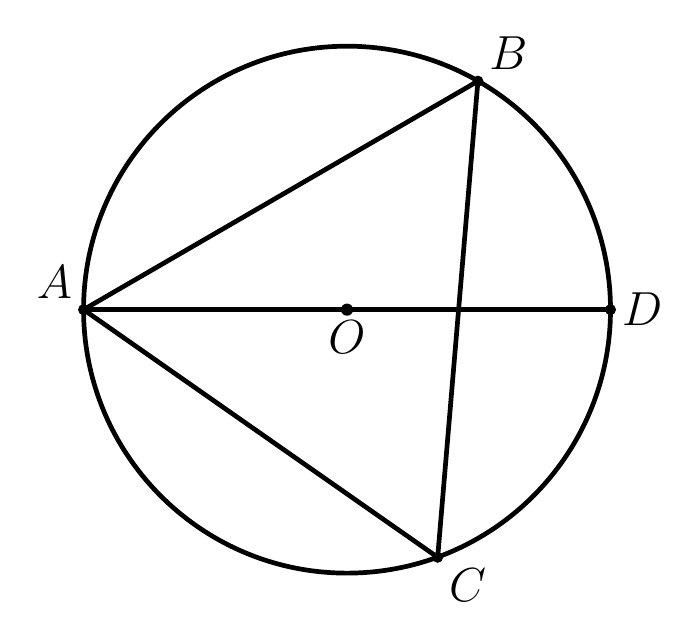
\begin{tikzpicture}[line width=1.7pt, line join=round]
  % Named coordinates (converted from pixels, y flipped)
  \coordinate (O) at (0,0);
  \coordinate (A) at (-3.346,0);
  \coordinate (D) at (3.346,0);
  \coordinate (B) at (1.662,2.902);
  \coordinate (C) at (1.151,-3.145);

  % Circle (solid, black)
  \draw[black] (O) circle[radius=3.346];

  % Chords and diameter (solid)
  \draw (A) -- (B);
  \draw (A) -- (C);
  \draw (B) -- (C);
  \draw (A) -- (D);

  % Labels
  \node[above left]  at (A) {\fontsize{17.5}{21}\selectfont $A$};
  \node[above right] at (B) {\fontsize{17.5}{21}\selectfont $B$};
  \node[below right] at (C) {\fontsize{17.5}{21}\selectfont $C$};
  \node[right]       at (D) {\fontsize{17.5}{21}\selectfont $D$};
  \node[below]       at (O) {\fontsize{17.5}{21}\selectfont $O$};

  % Filled dots (after labels, per critic)
  \fill (A) circle (2pt);
  \fill (B) circle (2pt);
  \fill (C) circle (2pt);
  \fill (D) circle (2pt);
  \fill (O) circle (2.2pt);
\end{tikzpicture}
\end{document}